%%%%%%%%%%%%%%%%%%%%%%%%%%%%%%%%%%%%%%%%%%%%%%%%%%%%%%%%%%%%%%%%%%%%%%
% Document preamble
\documentclass[10pt,letterpaper]{article}
\usepackage{fullpage}
\usepackage[top=1cm, bottom=3.5cm, left=1cm, right=1cm]{geometry}
\usepackage{amsmath,amsthm,amsfonts,amssymb,amscd}
\usepackage{lastpage}
\usepackage{enumerate}
\usepackage{fancyhdr}
\usepackage{mathrsfs}
\usepackage[usenames,dvipsnames]{xcolor}
\usepackage{graphicx}
\usepackage{listings}
\usepackage{courier}
\usepackage{longtable}
\usepackage{caption}
\usepackage{multicol}
\usepackage{hyperref}
\usepackage{amsmath}
\hypersetup{
    colorlinks=true,
    linkcolor=blue,
    filecolor=magenta,      
    urlcolor=blue}

\usepackage{geometry}
 \geometry{
 a4paper,
 total={170mm,257mm},
 left=20mm,
 right=20mm,
 top=20mm,
 }

\setlength{\parindent}{0.0in}
\setlength{\parskip}{0.05in}
\pagestyle{fancyplain}
\headheight 35pt
\lhead{\today}

%\footskip 35pt
\lfoot{}
\cfoot{}
\rfoot{Page \thepage \hspace{1pt} of \pageref{LastPage}}
\headsep 1.5em

\lstdefinelanguage{AMPL}{keywords={reset,set,model,data,param,var,arc,integer,minimize,maximize,subject,to,node,sum,in,Current,complements,integer,solve_result_num,IN,contains,less,suffix,INOUT,default,logical,sum,Infinity,dimen,max,symbolic,Initial,div,min,table,LOCAL,else,option,then,OUT,environ,setof,union,all,exists,shell_exitcode,until,binary,forall,solve_exitcode,while,by,if,solve_message,within,check,in,solve_result},sensitive=true,comment=[l]{\#}}

\lstset{language=AMPL,
        showstringspaces=false,
        basicstyle=\fontsize{7}{7}\ttfamily,
        numbers=none,
        keywordstyle=\bfseries,
        commentstyle=\textit,
        }
\renewcommand{\ttdefault}{pcr}

\newcommand{\obar}[1]{\mkern 2mu\overline{\mkern-2mu#1\mkern-2mu}\mkern 2mu}
\newcommand{\ubar}[1]{\mkern 2mu\underline{\mkern-2mu#1\mkern-2mu}\mkern 2mu}

% Edit these as appropriate
\chead{\textbf{\Large Spacecraft Model Design Description}}
\rhead{}


%%%%%%%%%%%%%%%%%%%%%%%%%%%%%%%%%%%%%%%%%%%%%%%%%%%%%%%%%%%%%%%%%%%%%%
% Begin document
\begin{document}
\tableofcontents
\newpage
\section{Model Introduction}
The Spacecraft Model's intention is to create model based estimates for key metrics associated with the design of an asteroid mining spacecraft. 
These metrics include, but are not limited to:
\begin{itemize}
    \item Dry mass
    \item Spacecraft cost
    \item Energy use
    \item Stay time
    \item Propellant usage
\end{itemize} 
These outputs are tightly correlated and cannot be solved for in isolation. This document will elaborate on how the Spacecraft Dry Mass is determined. 
The other output parameters, as mentioned, are closely correlated to the dry mass and their calculations can be easily inferred.
\newline
\autoref{fig-model-structure} describes how the dry mass model was broken down. This document will follow a similar structure for consistency. 

\begin{figure}[htb]
    \centering
    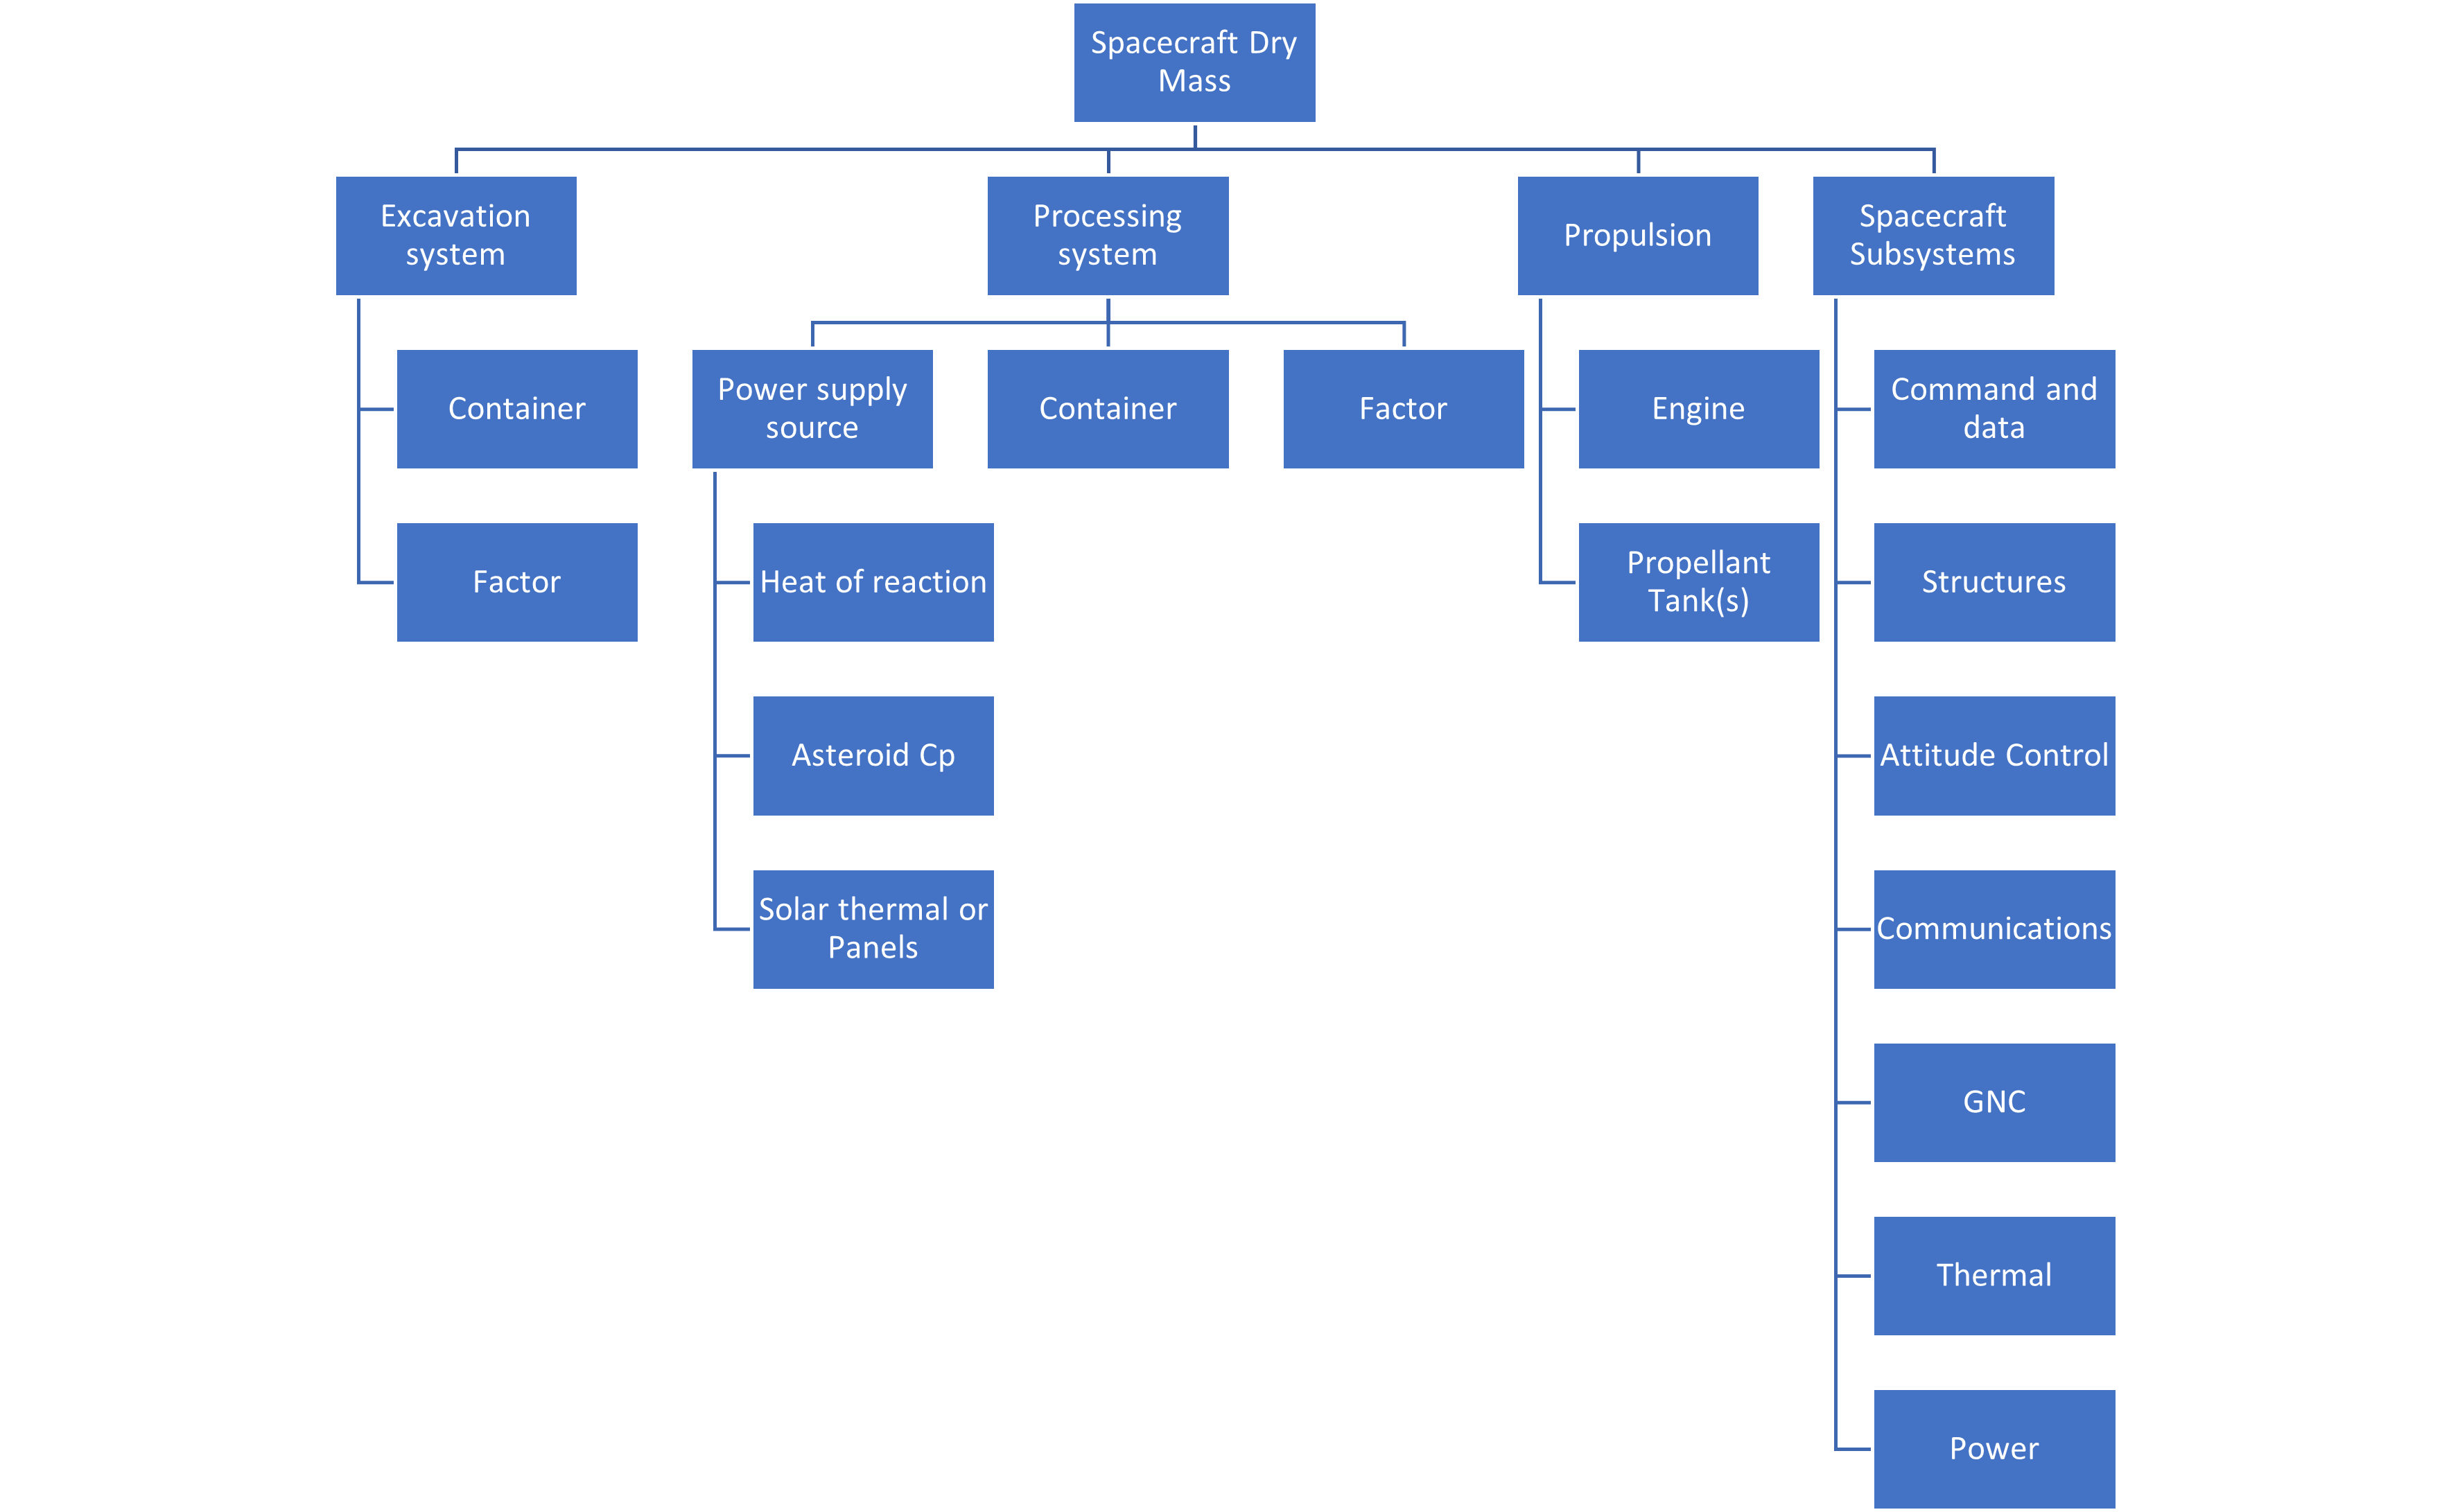
\includegraphics[width=0.9\linewidth]{mass structure.png}
    \caption{Spacecraft model structure for detemining dry mass.}
    \label{fig-model-structure}
\end{figure}



\newpage
\section{Excavation System Mass}
The general function of an excavation system is to interact with an asteroid, contain an amount of asteroid material, and deliver that material to a processing system. There are numerous ways to accomplish this task, such as having separate small excavation spacecrafts gather asteroid material and deliver it to a mother processing spacecraft. However, from a first principals modelling viewpoint the specifics of the excavation method are not particularly relevant. 
\newline
This model assumes a single, large container is used to interact with the asteroid and contain the asteroid material. This is the principal component of the excavation system. Motors, material transfer mechanisms, and other auxiliary equipments are modelled by a constant mass offset and a linear margin.
\newline 
The first calculation is to determine the amount of asteroid material the excavation system needs to gather. This model is based on processing water, so a target water mass in kg is the initial input. Some variable names have been changed from what they are in the python model for readability and clarity in this document. 
\begin{equation}
    m_{asteroid} = m_{waterTarget} / x_{asteroid water percent}
\end{equation}

This mass needs to be converted into a volume:
\begin{equation}
    V_{asteroid} = m_{asteroid} / density_{asteroid}
\end{equation}

It may be more practical to have an excavation system that takes several excavation passes at the asteroid. This would allow for a lower overhead excavation system volume and mass.
\begin{equation}
    V_{excavation} = V_{asteroid} / n_{number of excavation scoops}
\end{equation}

The shape of the excavation container (cube, cylinder, sphere) determines the relationship between the contained volume and the surface area needed to contain that volume. This relationship is modelled below:
\begin{equation}
    SA/V = SAtoV_{factor} / V_{excavation}^{1/3}
\end{equation}
\begin{equation}
    SA_{excavation} = SA/V \cdot V_{excavation}
\end{equation}

The surface area needed to contain the asteroid material is used to calculate the mass of the excavation container.
\begin{equation}
    m_{excavationContainer} = SA_{excavation} \cdot material_{thickness} \cdot material_{density}
\end{equation}

The total mass of the excavation system is then 
\begin{equation}
    m_{excavation} = m_{excavation offset} + m_{container} \cdot containerMass_{factor}
\end{equation}

The output to these equations over a range of water targets is shown in \autoref{fig-exmass}. The inputs are varied within the larger model, this figure is meant to show the deterministic model behavior with respect to excavation mass.
\begin{figure}[htb]
    \centering
    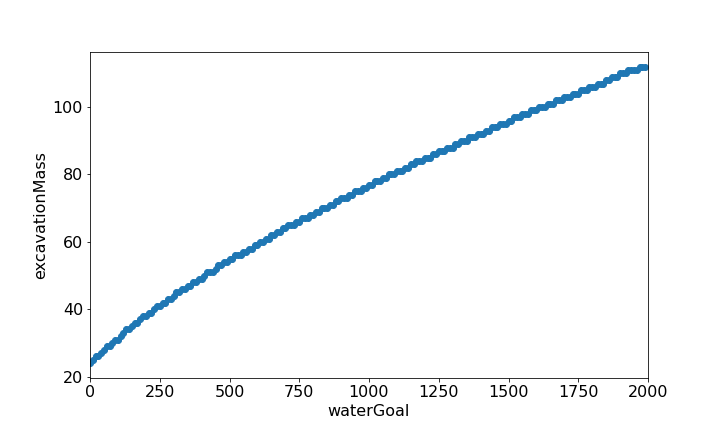
\includegraphics[width=0.5\linewidth]{exMass_vs_waterGoal.png}
    \caption{Excavation mass calculation for range of target water masses. Both values are in kilograms.}
    \label{fig-exmass}
\end{figure}

\newpage
\section{Processing System Mass}
The function of the processing system is to receive asteroid material from the excavation system and process it into pure water.
At the time of writing this, there is no system within the model that purifies the water, it is therefore assumed the output of initial processing is pure water. This is likely an invalid assumption that needs to be corrected.
The main components of the processing system are a container to house the asteroid material and a power source to convert the asteroid material into water. The processing container volume is given by:
\begin{equation}
    V_{processing} = V_{excavation} / n_{processingNumberBatches}
\end{equation}
\begin{equation}
    m_{asteroidProcessing} = V_{processing} / density_{asteroid}
\end{equation}
as there is no need for the processing system to work on the same mass scale as the excavation system. The Processing container mass is calculated the same as the excavation container mass using equations 4-6. There are separate parameters for each system in the model to decouple the excavation system design from the processing system design. Additionally, in some architectures the processing could be done in the excavation container. This can easily be accomplished by setting the processing material density to 0.
\newline
The bulk of the processing system mass comes from the power needed to transform the asteroid material into water. The dehydration reaction takes place at 600C. All power and energy calculations are done on a per batch basis.
\begin{equation}
    E_{thermal} = Cp_{asteroid} \cdot (T_{end} - T_{start}) \cdot m_{asteroidProcessing}
\end{equation}
\begin{equation}
    E_{reaction} = H_{reaction} \cdot frac{m_{asteroidProcessing} / x_{asteroidWaterPercent}}{0.01802} 
\end{equation}
\begin{equation}
    E_{total} = E_{thermal} + E_{reaction}
\end{equation}
The total power of the system is calculated by dividing the total energy by the processing time. The processing time, in days, is an input to the model.
\begin{equation}
    P_{batch} = E_{total} / t_{processing} \cdot (1/24)(1/60)(1/60)
\end{equation}
Since the model uses processing time as an input, the design confirms to meet the specified processing times. Therefore, the time should be consistent no matter the amount of water being harvested. This is shown and confirmed in \autoref{fig-processTime}
\begin{figure}[htb]
    \centering
    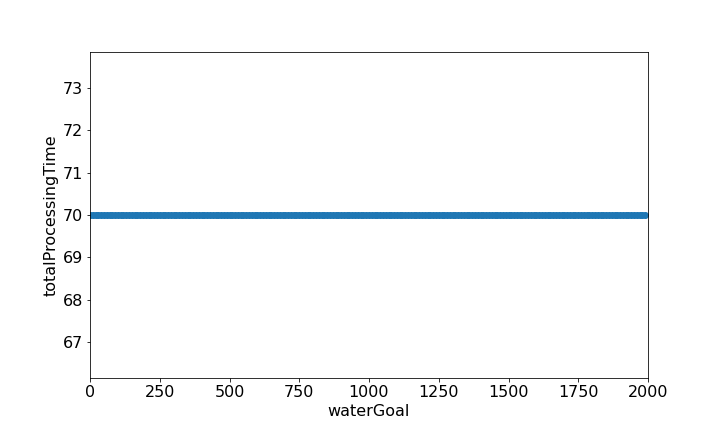
\includegraphics[width=0.5\linewidth]{processTime_vs_waterGoal.png}
    \captionsetup{justification=centering,margin=2cm}
    \caption{Processing time (days) over a range of water targets. The model treats processing time as an input variable, so the constant nature of this graph is expected}
    \label{fig-processTime}
\end{figure}


The total energy required for the processing system is shown in \autoref{fig-processingEnergy}.
\begin{figure}[htb]
    \centering
    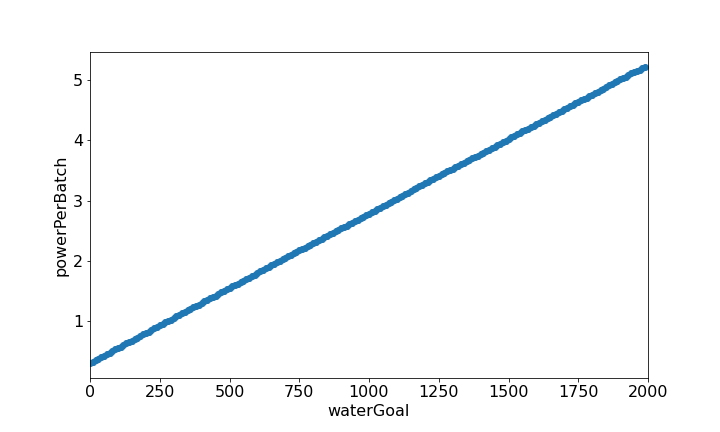
\includegraphics[width=0.5\linewidth]{powerPerBatch_vs_waterGoal.png}
    \caption{Processing energy (kW) per batch for a range of water targets (kg). }
    \captionsetup{justification=centering,margin=2cm}
    \label{fig-processingEnergy}
\end{figure}

The energy can come from two different ways: solar thermal power or through converting electricity to heat. The base assumption in the model is that solar panels will be used to produce electricity, and that will be turned into heat energy for processing the asteroid material. The energy density inputs can be easily changed to assess a different energy source, such as solar thermal concentrators. 
\begin{equation}
    m_{solarPanels} = \frac{P_{batch}}{SolarPanel_{EnergyDensity}\cdot e_{electricityToHeat} \cdot \frac{1}{r_{asteroidToSun}^2} \cdot (1 - SolarPanel_{degradation})^{designYears}}  
\end{equation}

The total processing mass is given by:
\begin{equation}
    m_{processing} = m_{container} \cdot containerMass_{factor} + m_{solarPanels} 
\end{equation}
\begin{figure}[htb]
    \centering
    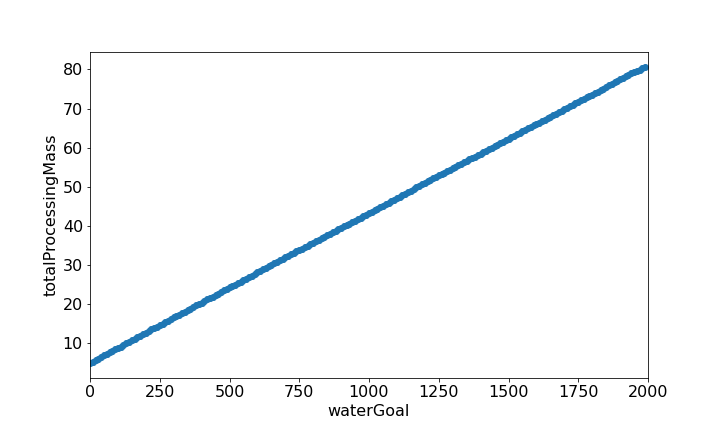
\includegraphics[width=0.5\linewidth]{processMass_vs_waterGoal.png}
    \captionsetup{justification=centering,margin=2cm}
    \caption{Processing mass (kg) over a range of water targets. Both values are in kilograms.}
    \label{fig-processMass}
\end{figure}

\newpage
\end{document}